\documentclass{article}

\title{\lr{Flight Dynamic II Bonus \#1}}

\author{علی بنی‌اسد 96108378}

\usepackage{lipsum}
\usepackage{fancyhdr}
\pagestyle{fancy}
\renewcommand{\sectionmark}[1]{%
	\markboth{\thesection\quad #1}{}}
\fancyhead{}
\fancyhead[R]{\leftmark}
\fancyhead[L]{علی بنی‌اسد 96108378}

\usepackage{graphicx}

\usepackage{xepersian}
\settextfont{B Nazanin}


\begin{document}
	\maketitle
	\section{مقدمه}
	در این گزارش ابتدا به بررسی تاربخچه اثر پرداخته می‌شود سپس به بررسی کارکرد آن از دیدگان مورخین پرداخته خواهد شد. 
	\begin{figure}[h!]
		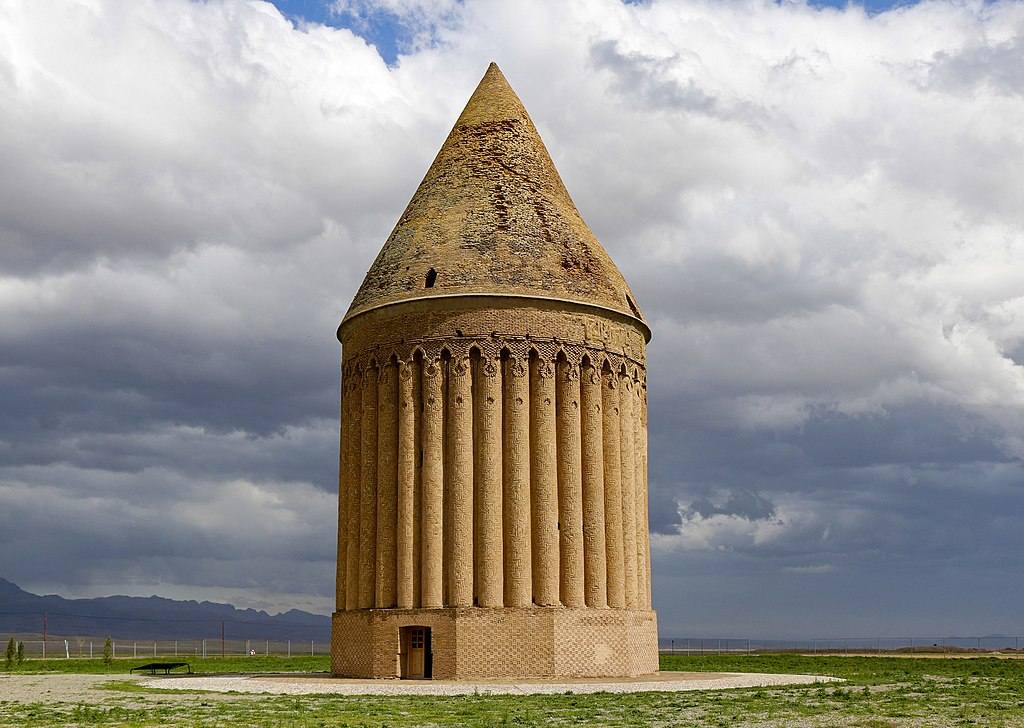
\includegraphics[width=\linewidth]{figures/Radkan_Tower,_Chenaran_2015-01-26.jpg}
		\caption{برج رادکان}
		\label{radkan}
	\end{figure}


در شکل \ref{radkan} نمایی از این برج آورده شده است. برج رادکان یک میل و بنای تاریخی است که در فاصله ۷۴ کیلومتری شمال مشهد و ۲۶ کیلومتری شمال غربی چناران واقع شده‌است. برج رادکان به ارتفاع ۲۵ متر، با بدنه استوانه‌ای و گنبد مخروطی شکل، اثری تاریخی مربوط به قرن هفتم هجری است. نمای خارجی بنا تا ارتفاع سه متری به صورت ۱۲ ضلعی و پس از آن تا زیر گنبد دارای ۳۶ ترک یا نیم استوانه بوده و داخل آن هشت ضلعی است.

\clearpage
برج رادکان چناران بر دشت میان توس و رادکان سایه افکنده و همتای دیگر آن نیز در کردکوی وجود دارد که به رادکان غربی مشهور است. همین موضوع باعث شده برخی نام رادکان را با راه و مسیر هم پیوند بدانند چنان‌که «راد» و «رد» در زبان پهلوی به معنای نظم و ترتیب و «رده» آمده و برج رادکان در مسیر راه و جاده درست همین کار را می‌کند که از نامش پیداست.
\section{معماری}
بلندای این برج ۳۵ متر، قطر داخلی‌اش ۱۴ متر و قطر خارجی آن ۲۰ متر می‌باشد. منظر بیرونی بنا تا ارتفاع ۵.۲ متری به شکل ۱۲ ضلعی و از آن جا تا زیر گنبد به صورت ۳۶ ترک نیم ستونی ساخته شده‌است. برج رادکان دارای گنبد مخروطی شکل است که ساختمان آن احتمالاً در سال ۶۰۷ قمری به پایان رسیده‌است. تاریخ احداث برج رادکان را ماکس افن برشم آلمانی سال ۶۰۰ و اندی و هرتسفلد سال ۶۸۰ ذکر کرده‌اند. هرتسفلد برج را مقبره یکی از حکام مغول می‌داند که برخی وی را امیر ارغون مغول می‌دانند. گدار مستشرق فرانسوی آن را آرامگاه یک زن و مطلع الشمس آن را از آثار دیلمی‌ها می‌داند. علاوه بر راهنمایی مسافران و مقبره به دلیل وجود منفذهایی به تعداد بروج دوازده‌گانه برخی برای این برج کارکرد تقویم و ستاره‌شناسی نیز قائل‌اند. برج رادکان، در روزگار اوج خود، تنها تعیین‌کننده فصل، سال و نوروز در جهان بوده‌است.

در مورد معمار و طراح این اثر اطاعات دقیقی وجود ندارد. در یعضی موارد طراحی برج را به احمد بن عمر نسب داده‌اند در حالی 
یعضی معتقداند این اثر شاهکار  خواجه نصیرالدین طوسی است.
\section{کارکرد}
پیشتر گفته شد گروهی معتقداند که این یک شاهکار طراحی است و از طرفی برخی دیگر می‌گویند بنای خاصی است ولی ولی هرگز یک شاهکار طراحی و ساخته خواجه نصیرالدین طوسی نبوده است. بر همین اساس عده‌ای کارکرد بسیار کمی به آن نسبت می‌دهد در حالی که گروه دیگر آن را در حد یک رسد خانه مانند سدس فخری می 
دانند.
		\begin{figure}[h!]
			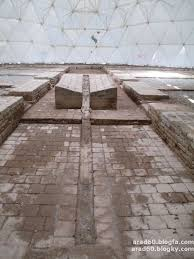
\includegraphics[width=50mm]{figures/sodos.jpeg}
			\centering
			\caption{بقایای رصدخانه سدس فخری}
			\label{sodos}
		\end{figure}
		\clearpage
	
	یکی از کاربردهای اصلی این بنا هر در گروه بیان شده آن را قبول دارند تعیین زمان زمستان و تابستان است. کارکرد آن به این صورت است که اگر در هنگام عصر خورشید در راستای این دریچه قرار گرفت تابستان است اگر هنگام صبح در این دریچه قرار گرفت زمستان است.
	\begin{figure}[h!]
			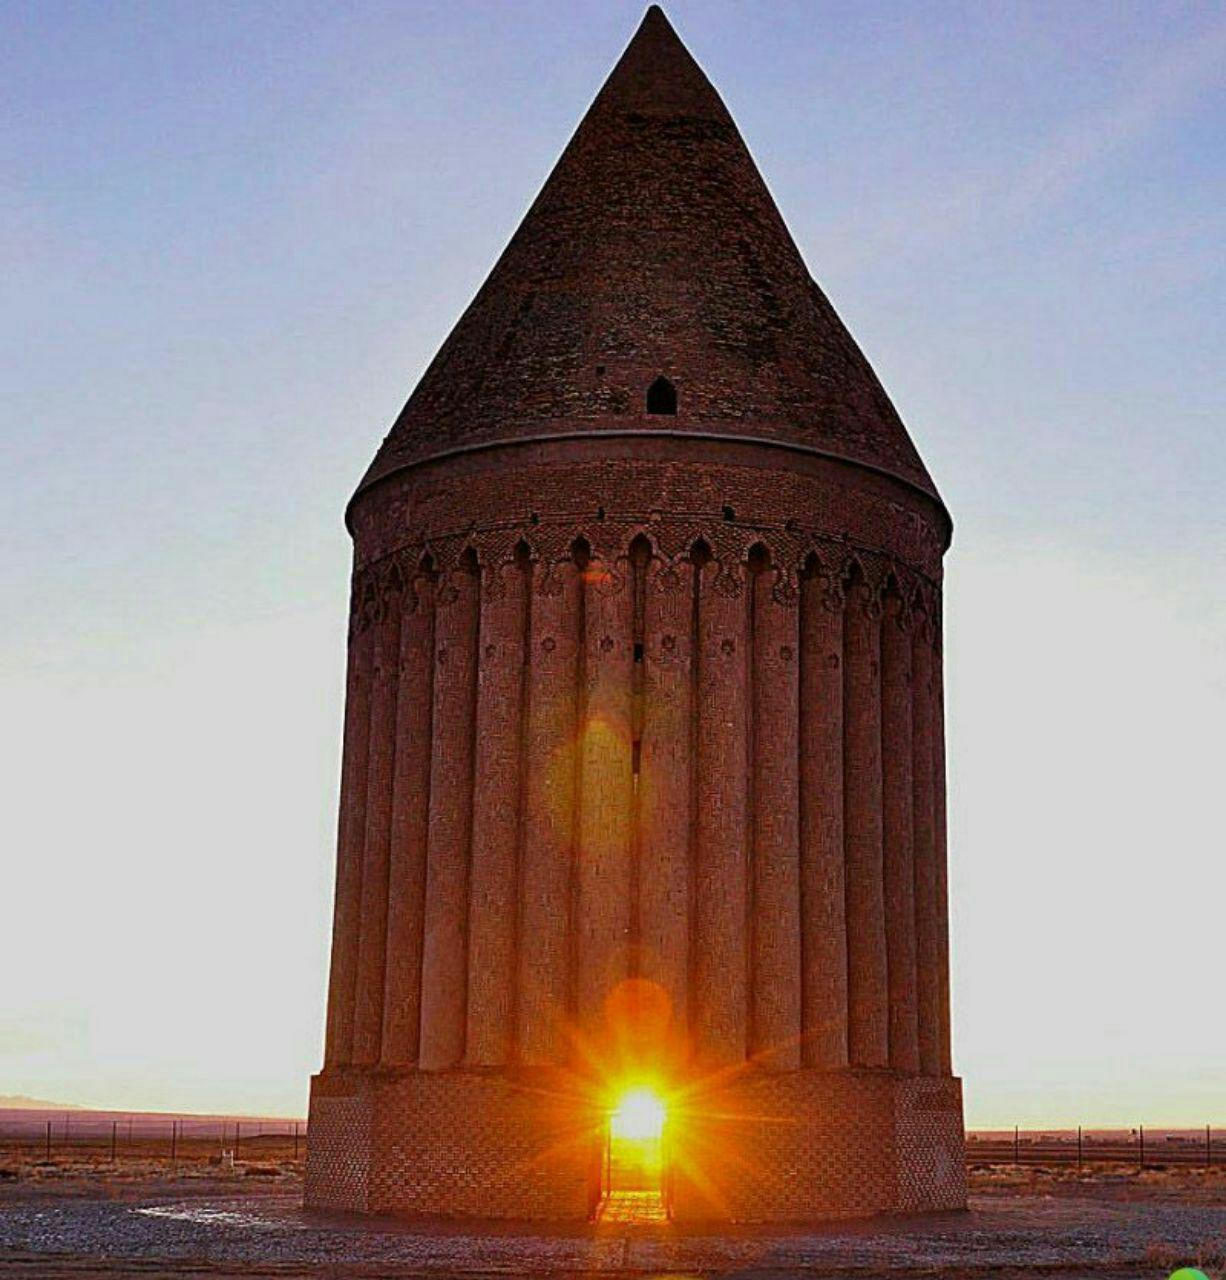
\includegraphics[width=\linewidth]{figures/radkan.jpg}
			\centering
			\caption{بقایای رصدخانه سدس فخری}
			\label{radkantaein}
		\end{figure}
		
		
		
	در شکل \ref{radkan}  این کاربرد آورده شده است که با توجه به طلوع و یا غروب آفتاب شروع فصل را تشخیص داد. این کارکرد بر اساس مشاهده هر حرکت خورشید و بدست آوردن مدلی برای حرکت ان بود. این معادلات بر اساس زمین مرکز انجام شدند ولی دقت بسیار بالایی داشتند. در آن زمان با توجه به پیشرفت علم برای ساخت یک بنا با این قابلیت نیاز به یک دانشمند بزرگ مانند خواجه نصیرالدین طوسی نبود و یک طلبه معمولی در آن زمان توانایی انجام این محاسبات را داشت. از طرفی بدون محاسبات و تنها با بررسی ساده الگو حرکت خورشید به راحتی می‌توان این بنا را ساخت.
	در مورد این اثر آقای منوچهر آرین تحقیقات بسیاری انجام داده است که البته به این تحقیقات نقدهای جدی وارد است که در ادامه به بررسی آنها پرداخته می شود.
	\clearpage
آقای آرین 	برج رادکان را بنایی می داند که می تواند با دقتی در حد یک سدس فخری لحظات اعتدالین و انقلابین را نشان دهد. سدس فخری ابزاری است که اولین بار خجندی آن را برای تعیین ارتفاع خورشید در لحظۀ ظهر حقیقی ابداع کرد. این ابزار از یک سدس دایرۀ عظیم مدرج ساخته است که نور خورشید از یک روزنه در مرکز دایره روی آن می افتد، اما برج رادکان مثل هر برج دیگری فاقد درجه بندی است. با این حال آقای آرین  معتقد است چون این برج دوازده دریچه دارد، نور خورشید از این دریچه ها وارد می شود و روی دیوارهای داخلی آن حرکت می کند و با مشخص کردن محل افتادن نور از این دریچه ها نه تنها می توان لحظات اعتدالین و انقلابین را 
بلکه آغاز تمام ماه های شمسی را یافت.
یک تأمل ساده نشان می دهد که حرکت پرتوهای داخل شده از پنجره ها و دریچه های تمام ساختمان های دنیا دارای چنین ویژگی ای هستند. پرتو نوری که از پنجره اتاق بنده در ساعت 10 صبح اول فروردین ماه وارد می شود، بر همان نقطه ای نمی افتد که ساعت 10 دوم فروردین می افتد و اگر آن نقطه را علامت بگذاریم سال بعد نیز در همان ساعت و همان روز پرتو نور در همان نقطه می افتد. ولی این باعث نمی شود که این ساختمان «رصدخانه» شود. نویسنده با علاقه ای مثال زدنی وقت بسیاری را صرف دنبال کردن این پرتوها داخل برج کرده و امروزه به لطف درجه بندی ها و نشانه گذاری های ایشان روی آجرهای داخلی برج، می توان بر اساس مسیر حرکت 
این نورها از برج رادکان به عنوان یک تقویم نجومی استفاده کرد. ولی می توان همین کار را در هر ساختمانی انجام داد و آن را به یک تقویم نجومی تبدیل کرد.
	\begin{figure}[h!]
			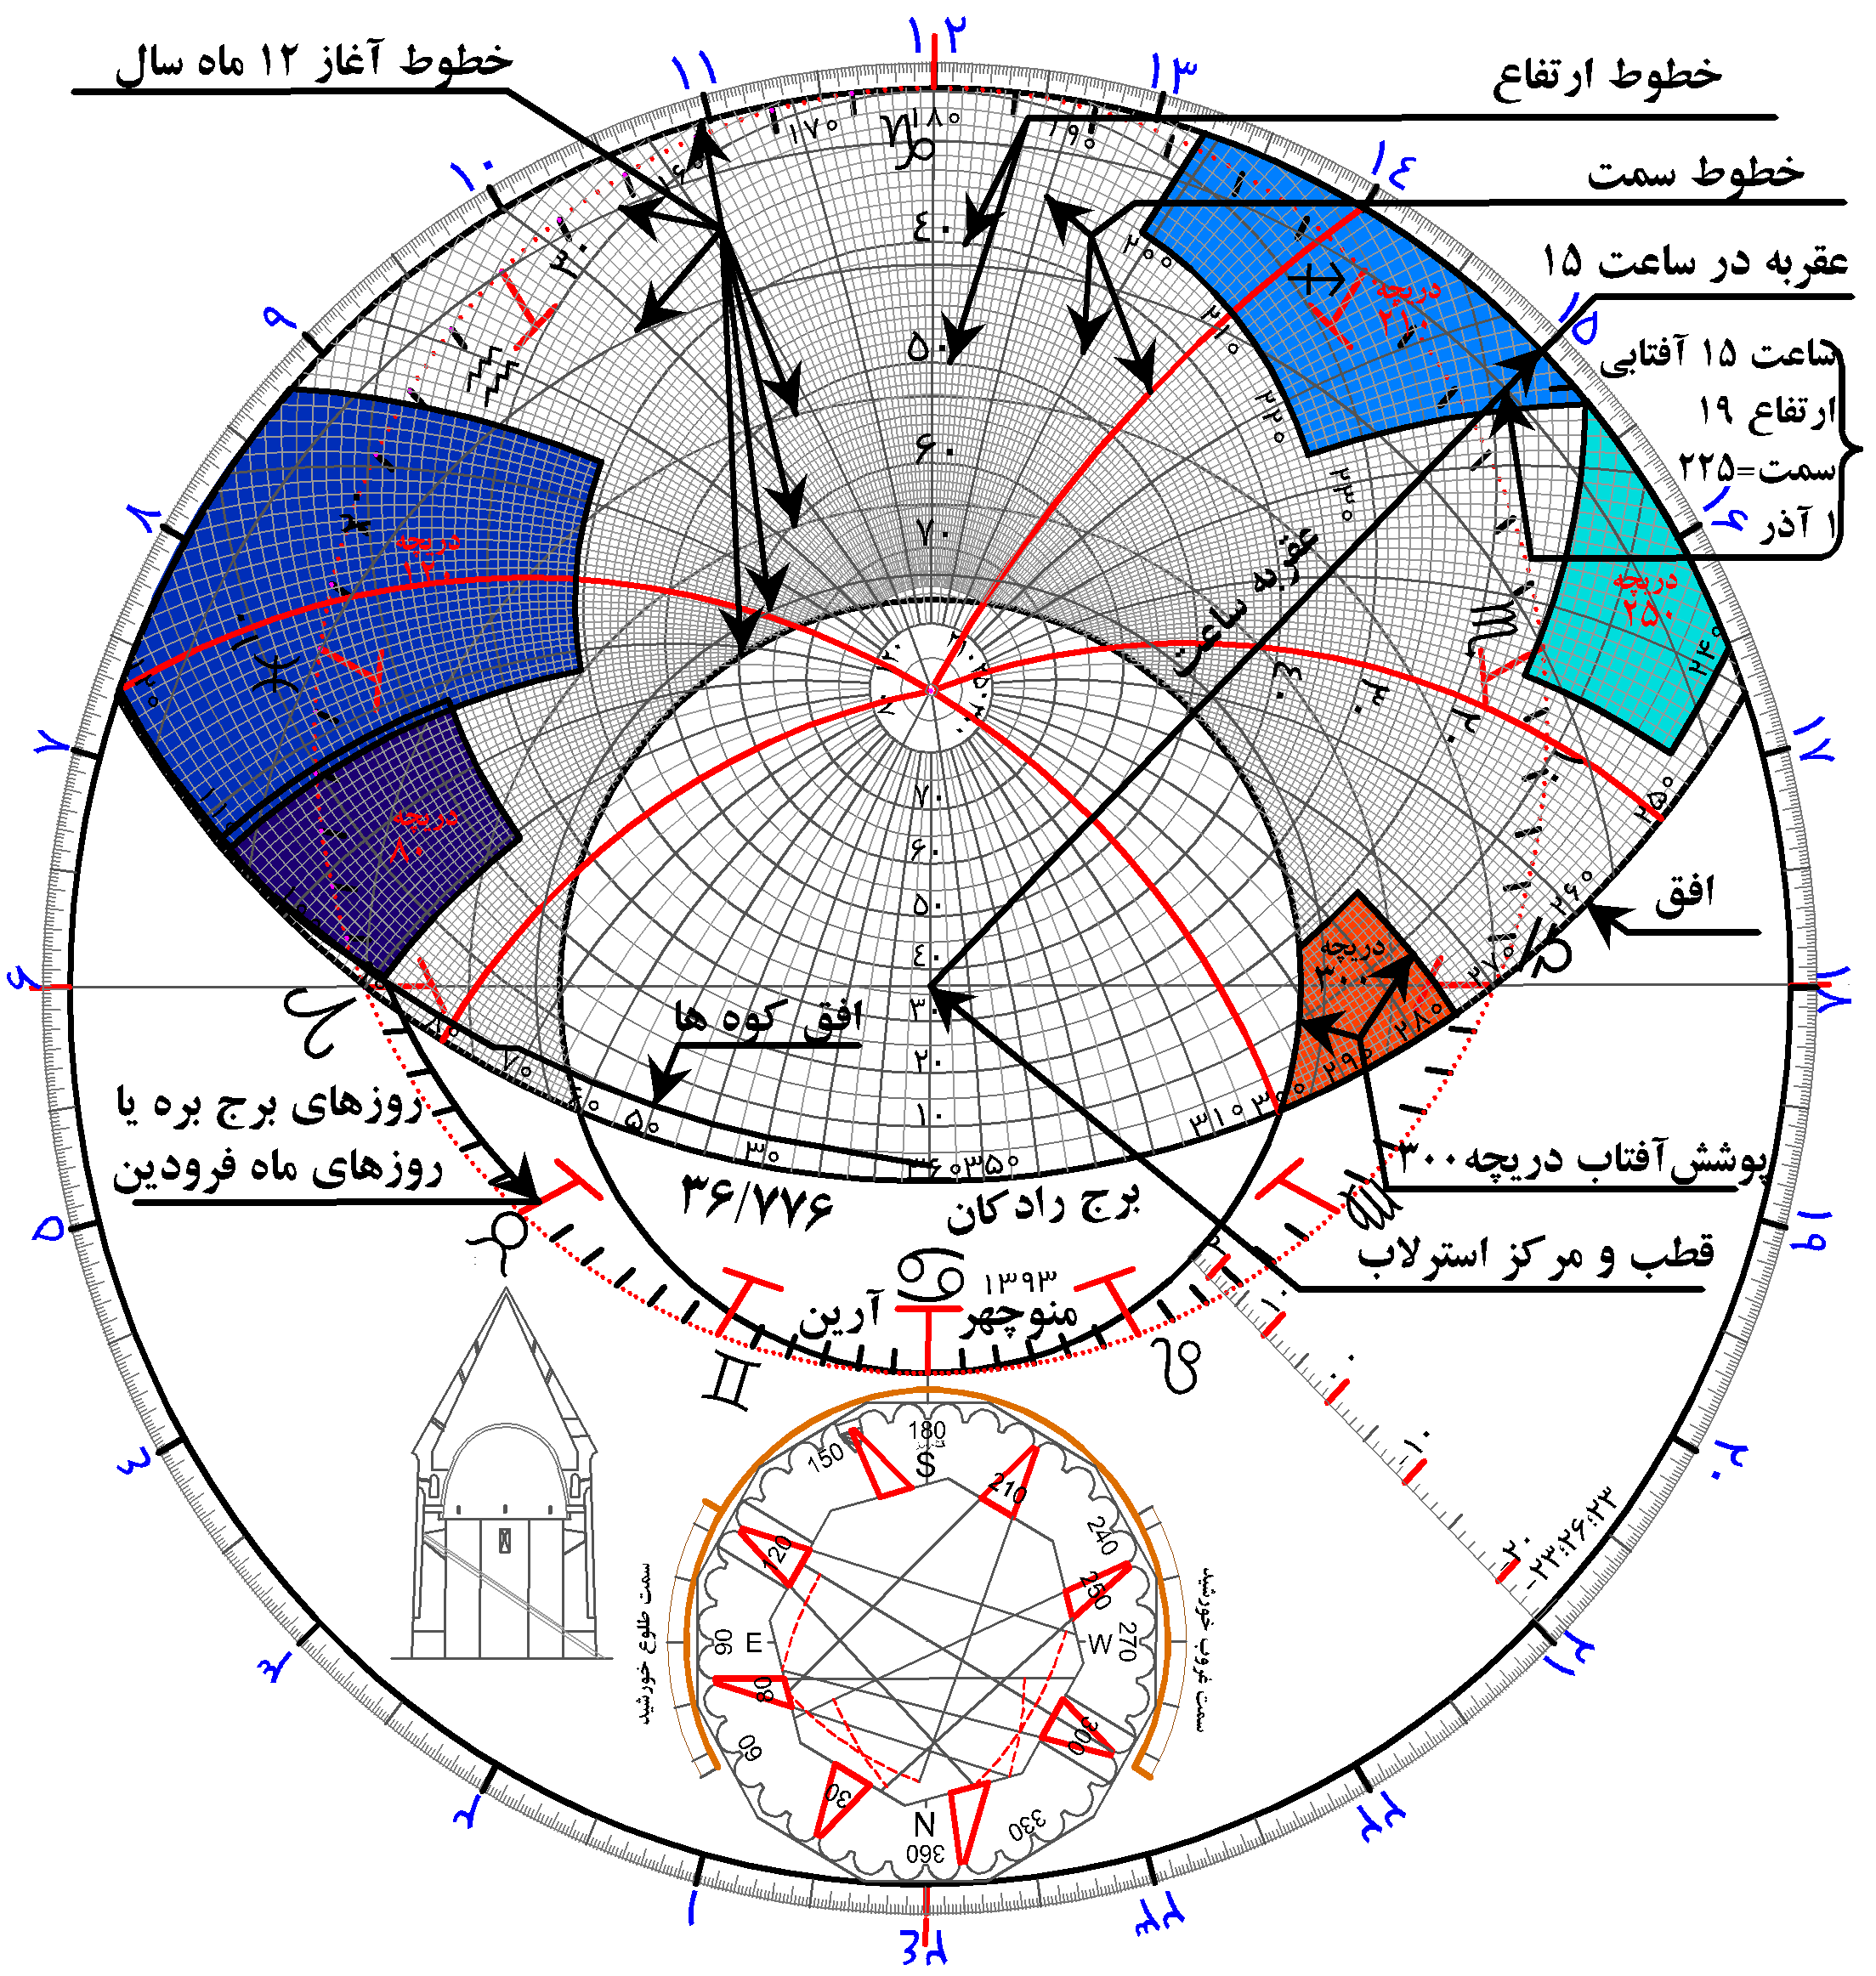
\includegraphics[width=\linewidth]{figures/r5.png}
			\caption{برج رادکان در قالب سدس}
			\label{radkandosos}
		\end{figure}
		\clearpage
		
	در شکل \ref{radkandosos} بر اساس تلاش‌های آقای آرین این برج را در قالب یک سدس بسیار پیشرفته آورده است که با توجه بر نور خورشید ورودی می‌توان ساعت، ماه  و دیگر موارد اشاره شده را تشخیص داد.   
\end{document}
